\documentclass[12pt]{article}
\usepackage{amsmath}
\usepackage{listings}
\usepackage{color}
\usepackage{graphicx}
\usepackage{bm}
\usepackage[margin=0.5in]{geometry}

\title{Homework 1}
\author{Dan Kolbman}
\date{November 17, 2014}

\definecolor{mygreen}{rgb}{0,0.6,0}
\definecolor{mygray}{rgb}{0.95,0.95,0.95}
\definecolor{mymauve}{rgb}{0.58,0,0.82}
%\definecolor{mygray}{RGB}{22, 22, 22}}

\lstset{ 
  language=Python,
  backgroundcolor=\color{mygray},   % choose the background color
  basicstyle=\footnotesize,        % size of fonts used for the code
  breaklines=true,                 % automatic line breaking only at whitespace
  captionpos=b,                    % sets the caption-position to bottom
  commentstyle=\color{mygreen},    % comment style
  %escapeinside={\%*}{*)},          % if you want to add LaTeX within your code
  keywordstyle=\color{blue},       % keyword style
  stringstyle=\color{mymauve},     % string literal style
  frame=L,
  xleftmargin=\parindent,
  showstringspaces=false
}
\begin{document}
  
  \maketitle
  %\lstinputlisting{Problem1.out}

  %\begin{figure}[h!]
  %  \centering
  %  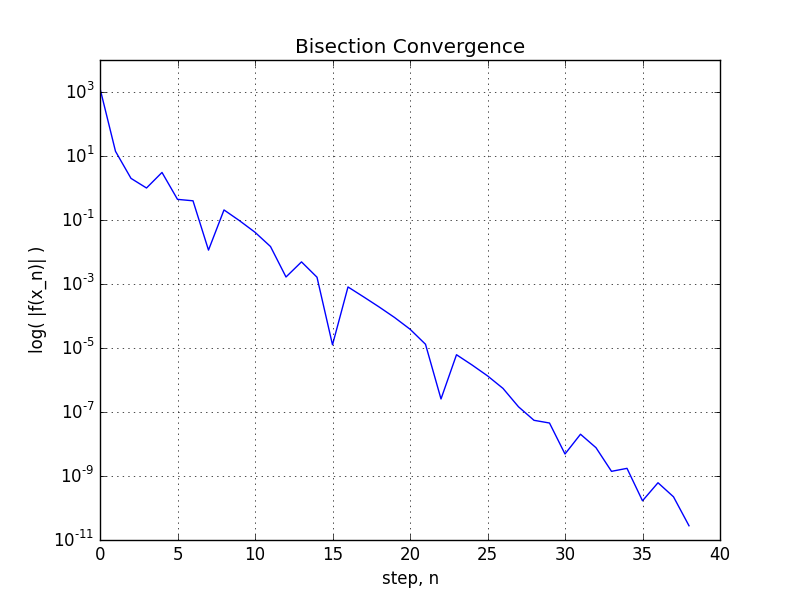
\includegraphics[width=0.5\textwidth]{Problem4a.png}
  %  \caption{(Approximately) Quadratic Convergence} %\end{figure}
 
  \section{Finite Differencing in Curved Coordinates}

  \section{Differentiation and Integration with Noise}


  \begin{align}
    f(x) &= sin(x)e^{cos(x)} \\
    f^{\prime}(x) &= (cos(x)-sin^2(x))e^{cos(x)}
  \end{align}

  \subsection{Differentiation using Stencils}
  \begin{figure}[h!]
    \centering
    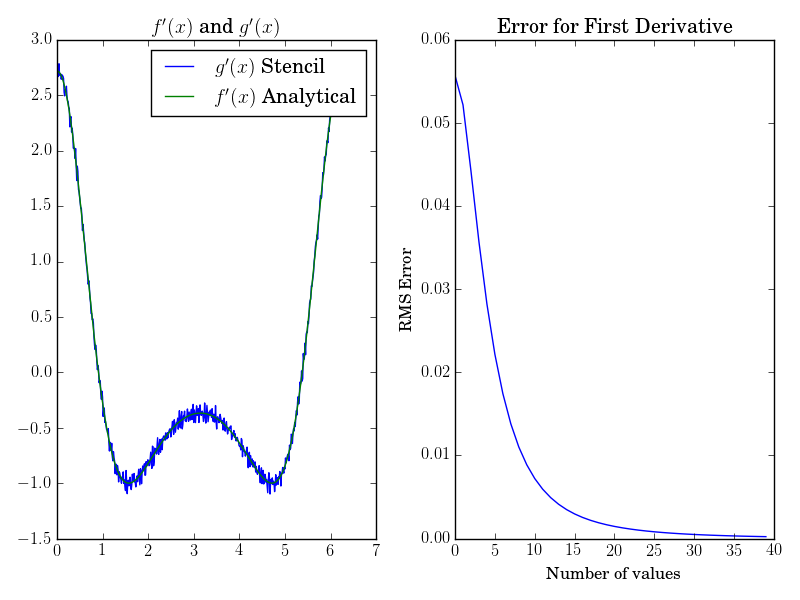
\includegraphics[width=0.8\textwidth]{Problem2ia.png}
    \caption{RMS Error in 5 point stencil for the first derivative}
  \end{figure}

  \begin{figure}[h!]
    \centering
    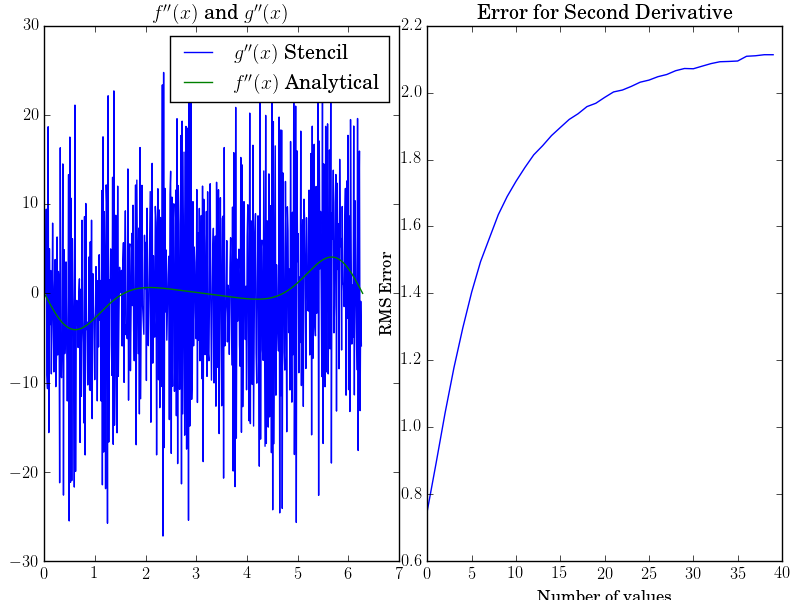
\includegraphics[width=0.8\textwidth]{Problem2ib.png}
    \caption{RMS Error in 5 point stencil for the second derivative}
  \end{figure}

  \subsection{Integration with Simpson's Rule}
  
  \begin{figure}[h!]
    \centering
    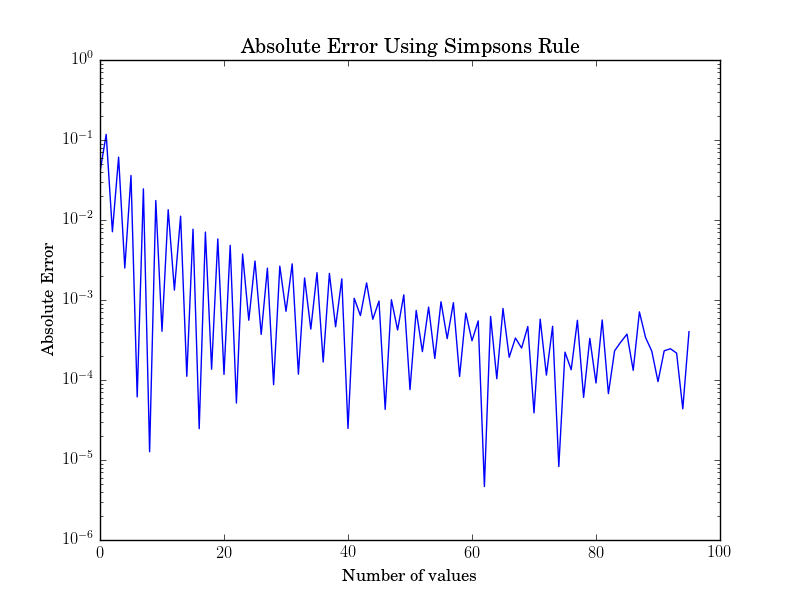
\includegraphics[width=0.8\textwidth]{Problem2ii.png}
    \caption{RMS Error using Simpson's Rule for varying numbers of points}
  \end{figure}

  \clearpage

  \section{Cepheid Lightcurve Integraiton}
  
  \begin{figure}[h!]
    \centering
    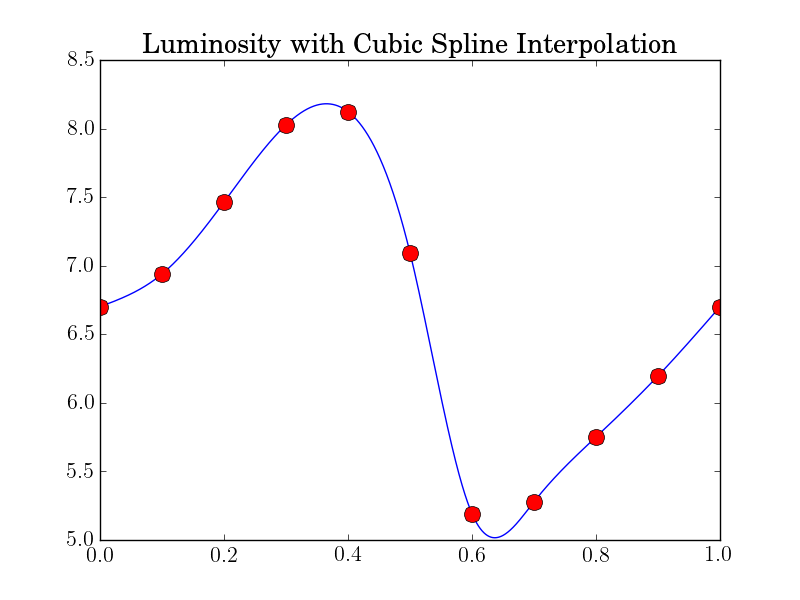
\includegraphics[width=0.8\textwidth]{Problem3.png}
    \caption{Magnitude converted to luminosity and interpolated with a cubic spline}
  \end{figure}

  \begin{table}[h!]
  \centering
  \begin{tabular}{ | c | c | c |}
    \hline
    Set Used  & Simpson's Rule & Trapezoid Method \\ \hline
    Data Only         & 6.0790 & 6.6789 \\
    Magnitude Spline  & 6.5974 & 6.5974 \\
    Luminosity Spline & 6.6725 & 6.6725 \\ \hline
  \end{tabular}
  \caption{Luminosity-days evaluted for different methods of integration}
  \end{table}

  \section{Planck's Law}
  $\nu$ was redefined to be dimensionless:
  $$\hat{\nu} \equiv \frac{h\nu}{k_BT}$$
  
  $\hat{\nu}$ was transformed to $tan(\hat{\nu}$ over the range $(0,\pi/2)$ to
  evaluate the integral over infinity.

  \subsection{Total Number Density}

  \begin{align}
    n_{tot} &= \frac{8\pi}{c^3}\frac{k_BT}{h}\int^{\infty}_0\hat{\nu}^2\frac{1}{e^{\hat{\nu}}-1}d\hat{\nu}\nonumber\\
      &= \frac{8\pi}{c^3}\frac{k_BT}{h}\int^{\pi/2}_0\frac{tan(\hat{\nu})}{cos(\hat{\nu})}^2\frac{1}{e^{\hat{\nu}}-1}d\hat{\nu}\nonumber\\
      &=   2.40406 \left(\frac{8\pi}{c^3}\frac{k_BT}{h}\right) \nonumber
  \end{align}

  \subsection{Median Energy}

  \begin{align}
    median &= \frac{1}{2}\frac{8\pi}{c^3}\frac{k_BT}{h}\int^{\infty}_0 n_{\nu}\hat{\nu}d\hat{\nu}\nonumber\\
      &=  1.31058 \left(\frac{8\pi}{c^3}\frac{k_BT}{h}\right)^2 \nonumber
  \end{align}

  \subsection{Mean Energy}
  
  Using the frequency:
  \begin{align}
    \bar{\nu} &= 1.09030 \left(\frac{k_BT}{h}\right) \nonumber
  \end{align}
  Using the wavelength:
  \begin{align}
    \bar{\lambda} &= 0.64494 \left(\frac{hc}{k_BT}\right) \nonumber
  \end{align}
  The product should be $c$:
  \begin{align}
    \left[0.64494 \left(\frac{hc}{k_BT}\right)\right]\left[1.09030 \left(\frac{k_BT}{h}\right)\right] &= 0.70319c \nonumber
  \end{align}
  Which it isn't (Error somewhere).
  

  \subsection{Standard Deviation}

  \begin{align}
    \sigma_{\nu} &= 0.64756 \left(\frac{k_BT}{h}\right) \nonumber
  \end{align}

  \clearpage

  \section{Romberg Integration}
  
  \begin{table}[h!]
  \centering
  \begin{tabular}{ | c | c | c |}
    \hline
    Function  & $R_{3,3}$ & Actual \\ \hline
    $cos^2(x)$          & 1.0118 & 1.4546 \\
    $xln(x+1)$          & 0.2454 & 0.3243 \\
    $sin^2(x)-2xsin(x)$ & -1.060 & 1.3667 \\ 
    $(xln(x))^{-1}$     & 0.4082 & 0.5266 \\ \hline
  \end{tabular}
  \caption{Integral approximations using Romberg integration}
  \end{table}

  \section{Gaussian Quadrature}
  
  \begin{align}
    a &= \frac{7}{15}   \nonumber \\
    b &= \frac{16}{15}  \nonumber \\
    c &= \frac{7}{15}   \nonumber \\
    d &= \frac{1}{15}   \nonumber \\
    e &= -\frac{1}{15}  \nonumber
  \end{align}

\end{document}
